En este caso las prueba que realizamos fueron temporales, con el objetivo de comprobar la complejidad exponencial en el peor caso. Para ello hicimos un programa en C++ para generar grafos aleatoreamente que no entren en los casos triviales, es decir que tengan alguna arista y que no sean completos. También agregamos la posibilidad de determinar probabilísticamente la cantidad de aristas del grafo.

Cuando fuimos probando con distintas instancias, pudimos ir comprobando que a partir de unos $70$ u $80$ nodos, el tiempo de ejecución se vuelve considerable, y luego de los $100$ ya supera el minuto (todo esto fue probado en una computadora hogareña).

A continuación adjuntamos un gráfico obtenido con grafos de $15$ a $80$ nodos (5 de cada uno), con una probabilidad para las aristas del $50\%$.

\begin{center}
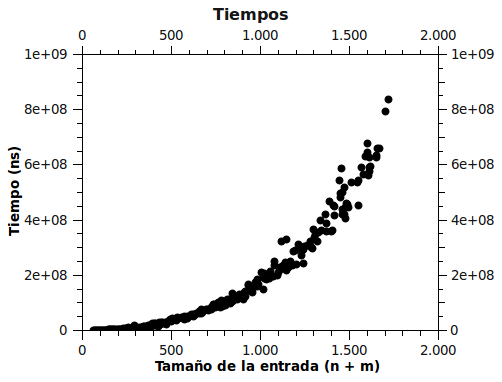
\includegraphics[scale=0.75]{img/exacto-tiempos.png} 
\end{center}

Cabe aclarar que al tomar las mediciones, hicimos tres corridas con los mismos datos de entrada y tomamos el mínimo de los tiempos de ejecución para cada instancia con el objetivo de disminuir los outliers. Igualmente hay bastantes, creemos que eso se puede deber a que el tiempo de ejecución es considerable, con lo cual puede ser que el scheduler del Sistema Operativo le de una prioridad baja y tenga que esperar.